\documentclass[conference]{IEEEtran}
\IEEEoverridecommandlockouts
% The preceding line is only needed to identify funding in the first footnote. If that is unneeded, please comment it out.
\usepackage{cite}
\usepackage{amsmath,amssymb,amsfonts}
\usepackage{algorithmic}
\usepackage{graphicx}
\usepackage{textcomp}
\usepackage{xcolor}
\usepackage{amsmath}
\usepackage{hyperref}
\def\BibTeX{{\rm B\kern-.05em{\sc i\kern-.025em b}\kern-.08em
    T\kern-.1667em\lower.7ex\hbox{E}\kern-.125emX}}
\begin{document}

\title{ANN-MPC and ILC on Building HVAC Control Systems
\thanks{Submitted as part of CMU 16745 course requirements. Github link of this project: \url{https://github.com/LW-G38/16745_final_project}}
}

\author{\IEEEauthorblockN{Wei Liang}
\IEEEauthorblockA{\textit{School of Architecture} \\
\textit{Carnegie Mellon University}\\
Pittsburgh, USA \\
weiliang@andrew.cmu.edu}
\and
\IEEEauthorblockN{Sizhe Ma}
\IEEEauthorblockA{\textit{Department of Civil and Environmental Engineering} \\
\textit{Carnegie Mellon University}\\
Pittsburgh, USA \\
sizhem@andrew.cmu.edu}
}

\maketitle

\begin{abstract}
Building heating, ventilation, and air conditioning (HVAC) systems are responsible to 20\% of the energy consumption in United States and take care of the thermal comfort of occupants.  It is of great benefit to develop and implement optimal control strategies to building HVAC systems. In this work, we propose a bi-level control design: for air handling unit (AHU), we propose a an Artificial Neural Network to train on simulated data based on model predictive control (MPC) structure. The final network/controller is able to directly interact with the system and imitate the performance of conventional MPC in some extent. At the bottom level, the temperature control of variable air volumes (VAVs) is achieved by an ILC controller design to ensure a close room air temperature set-point following without significant increase of the energy consumption. The results indicate an effectiveness of the the ILC algorithm by showing fast convergence property. The ILC design implemented on dynamic models trained and validated by real-world building HVAC data.
\end{abstract}

\begin{IEEEkeywords}
HVAC system, Model predictive control, Iterative learning control
\end{IEEEkeywords}

\section{Introduction}
Buildings are responsible for more than 40\% of energy consumption in the United States \cite{eia2021energy}. Within the sector, heating ventilation, and air conditioning (HVAC) systems consume up to 50\% of the energy use in U.S commercial and residential buildings \cite{capuano2019annual}. Despite their energy consumption, the primary function of building HVAC systems is to provide ideal indoor thermal conditions through temperature control. The thermal comfort for occupants in the built environments is essential as Americans spend more than 95\% of their time indoors \cite{bls2021indoor}. With the increased desire to minimize the energy consumption meanwhile maximize people's thermal comfort, it is of great benefit to develop and implement optimal control strategies to building HVAC systems.

A typical building HVAC system is shown in Fig. \ref{fig1}. On the top level, there is a single-duct air handling unit (AHU) where the supply air (SA) uses one single duct for both heating and cooling modes to the building. The AHU has one outside air (OA) inlet and one exhaust air (EA) outlet. In normal operation, the return air (RA) collected from room-level spaces in the building is drawn back to the AHU through the return fan. Part of RA is relieved out of the building as EA, the remainder of RA is recirculated through the mixing chamber to be mixed with OA. The proportion of recirculated air and OA is determined by the collective regulation of the outsider air damper, the exhaust air damper, and the economizer damper. After that, the mixed air (MA) goes through filters driven by the supply fan. The supply air is normally cooled down to 13 $^{\circ}$C (55$^{\circ}$F ) by the cooling coil and distributed to variable air volumes (VAVs) that directly discharge air to each room. The control problem at AHU level can be controlling supply air temperature, supply airflow rate, and the proportion between recirculate air and OA to satisfy the thermal and ventilation requirements of the building and reduce the energy cost. 

\begin{figure}[htbp]
\centerline{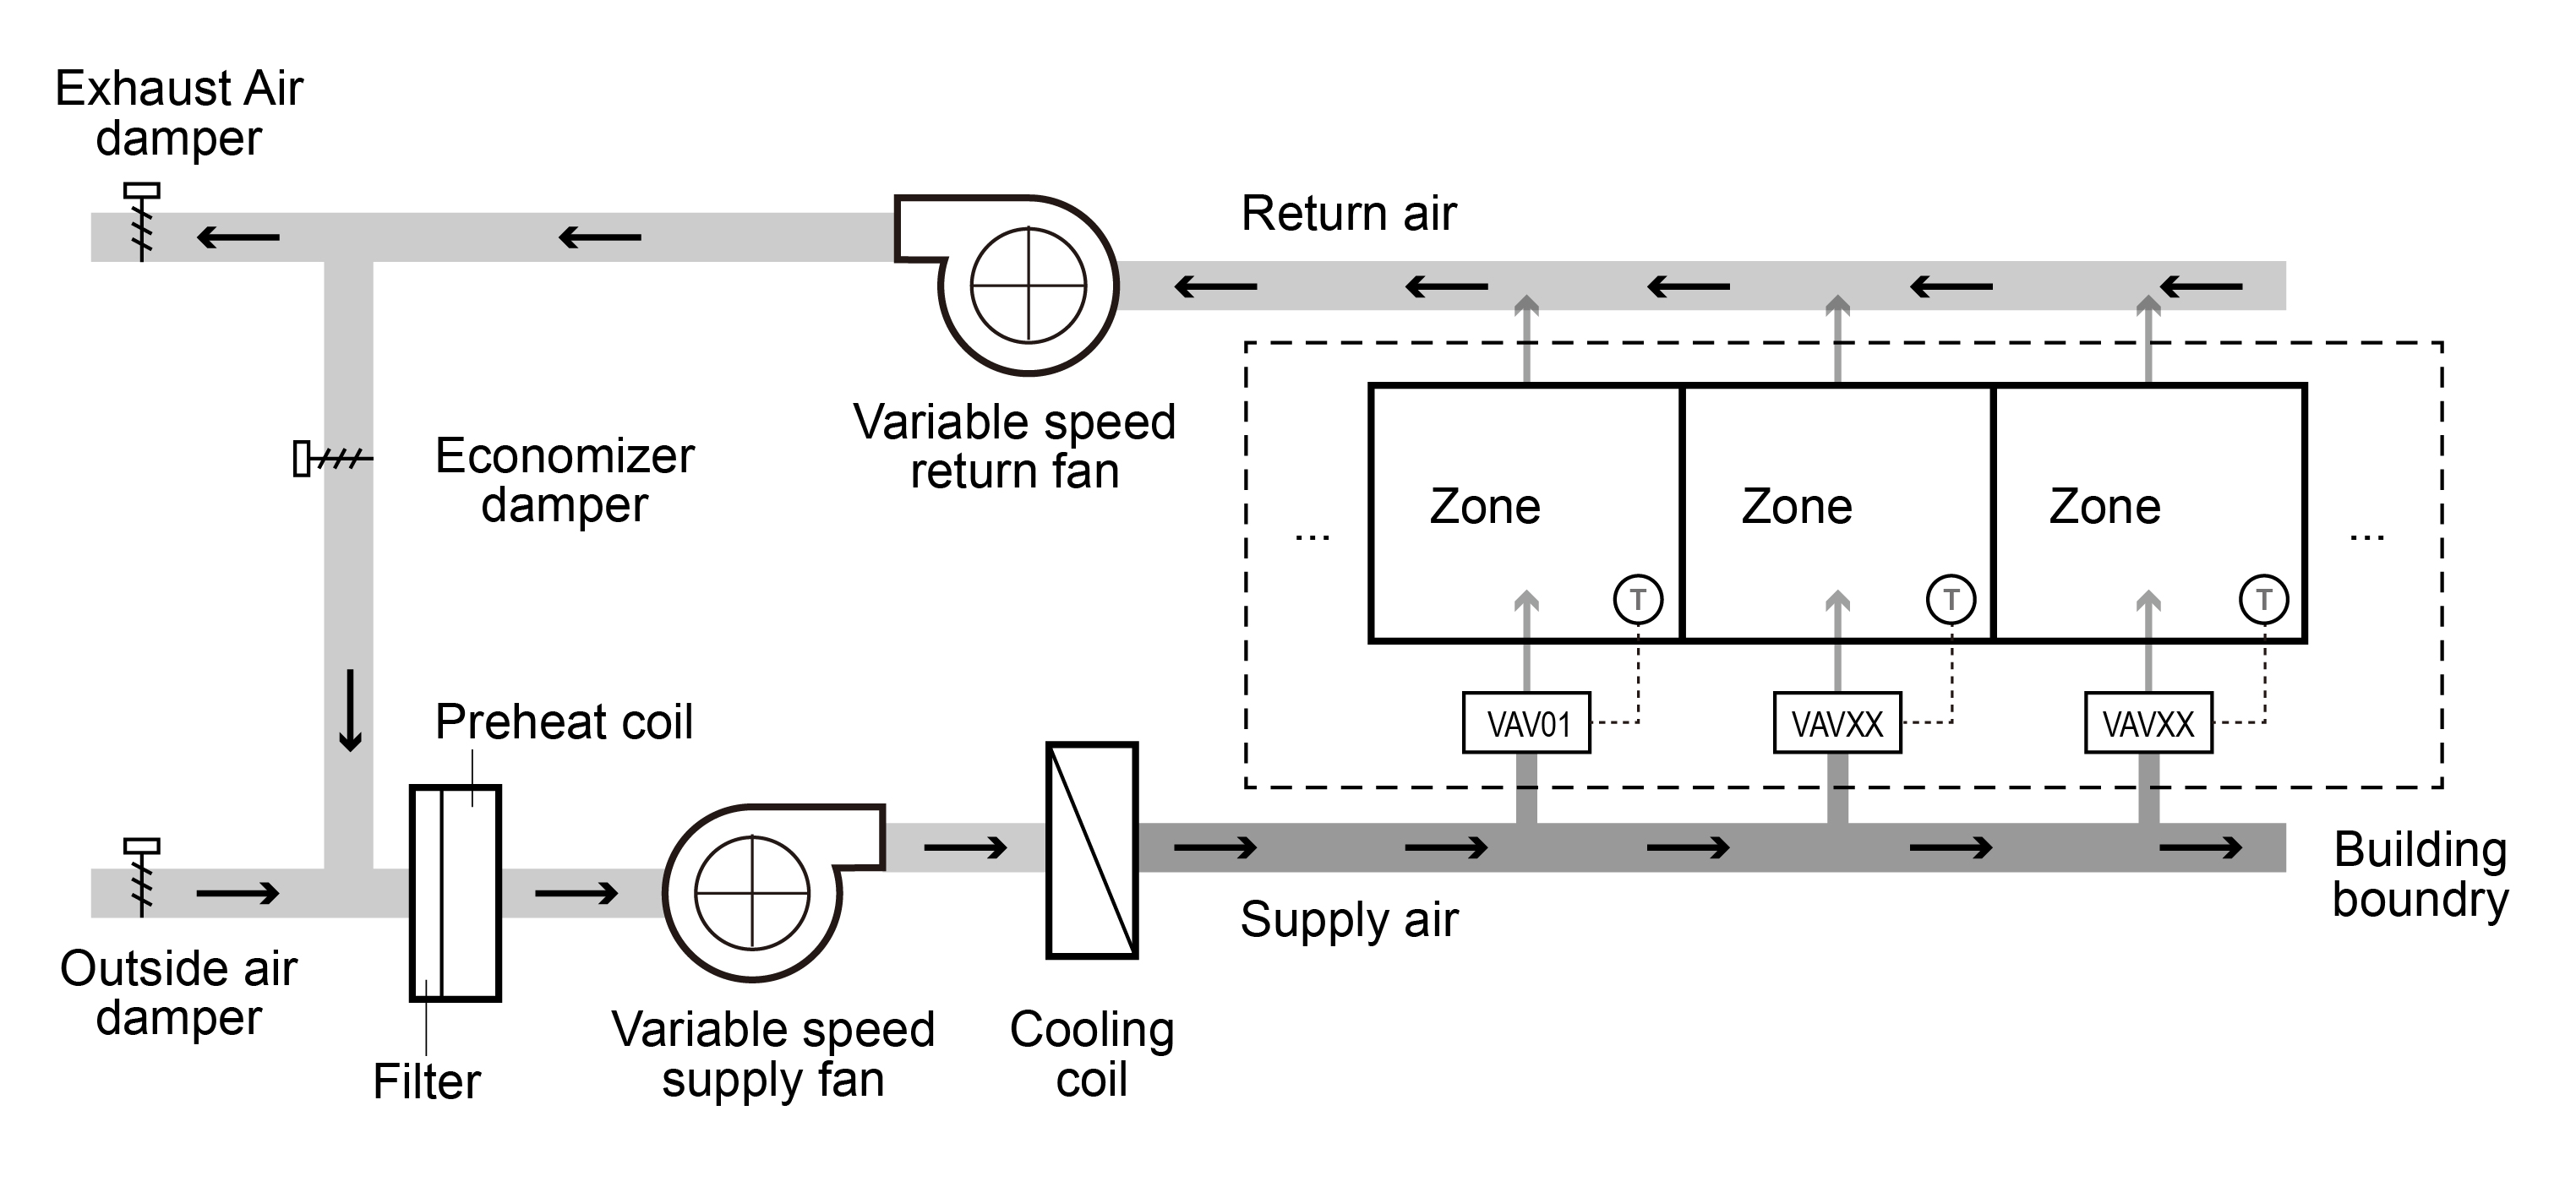
\includegraphics[width=0.5\textwidth]{Figures/AHU-VAV system.jpeg}}
\caption{A typical diagram for a single duct AHU-VAV system.}
\label{fig1}
\end{figure}

At the distributed level, a single duct terminal VAV box contains a control damper and a reheat coil, as shown in Fig. \ref{fig2}. When SA from AHU passes through a VAV, the control damper regulates the mass flow rate and the reheat coil will adjust the temperature of SA to ensure that the mass flow rate and the discharged air temperature to the room. This setup allows localized flow rate and temperature control for each thermal zones. In common practice, the VAV controller reads the temperature set-point from the thermostat located in the room to modulate the damper and reheat coil.

\begin{figure}[htbp]
\centerline{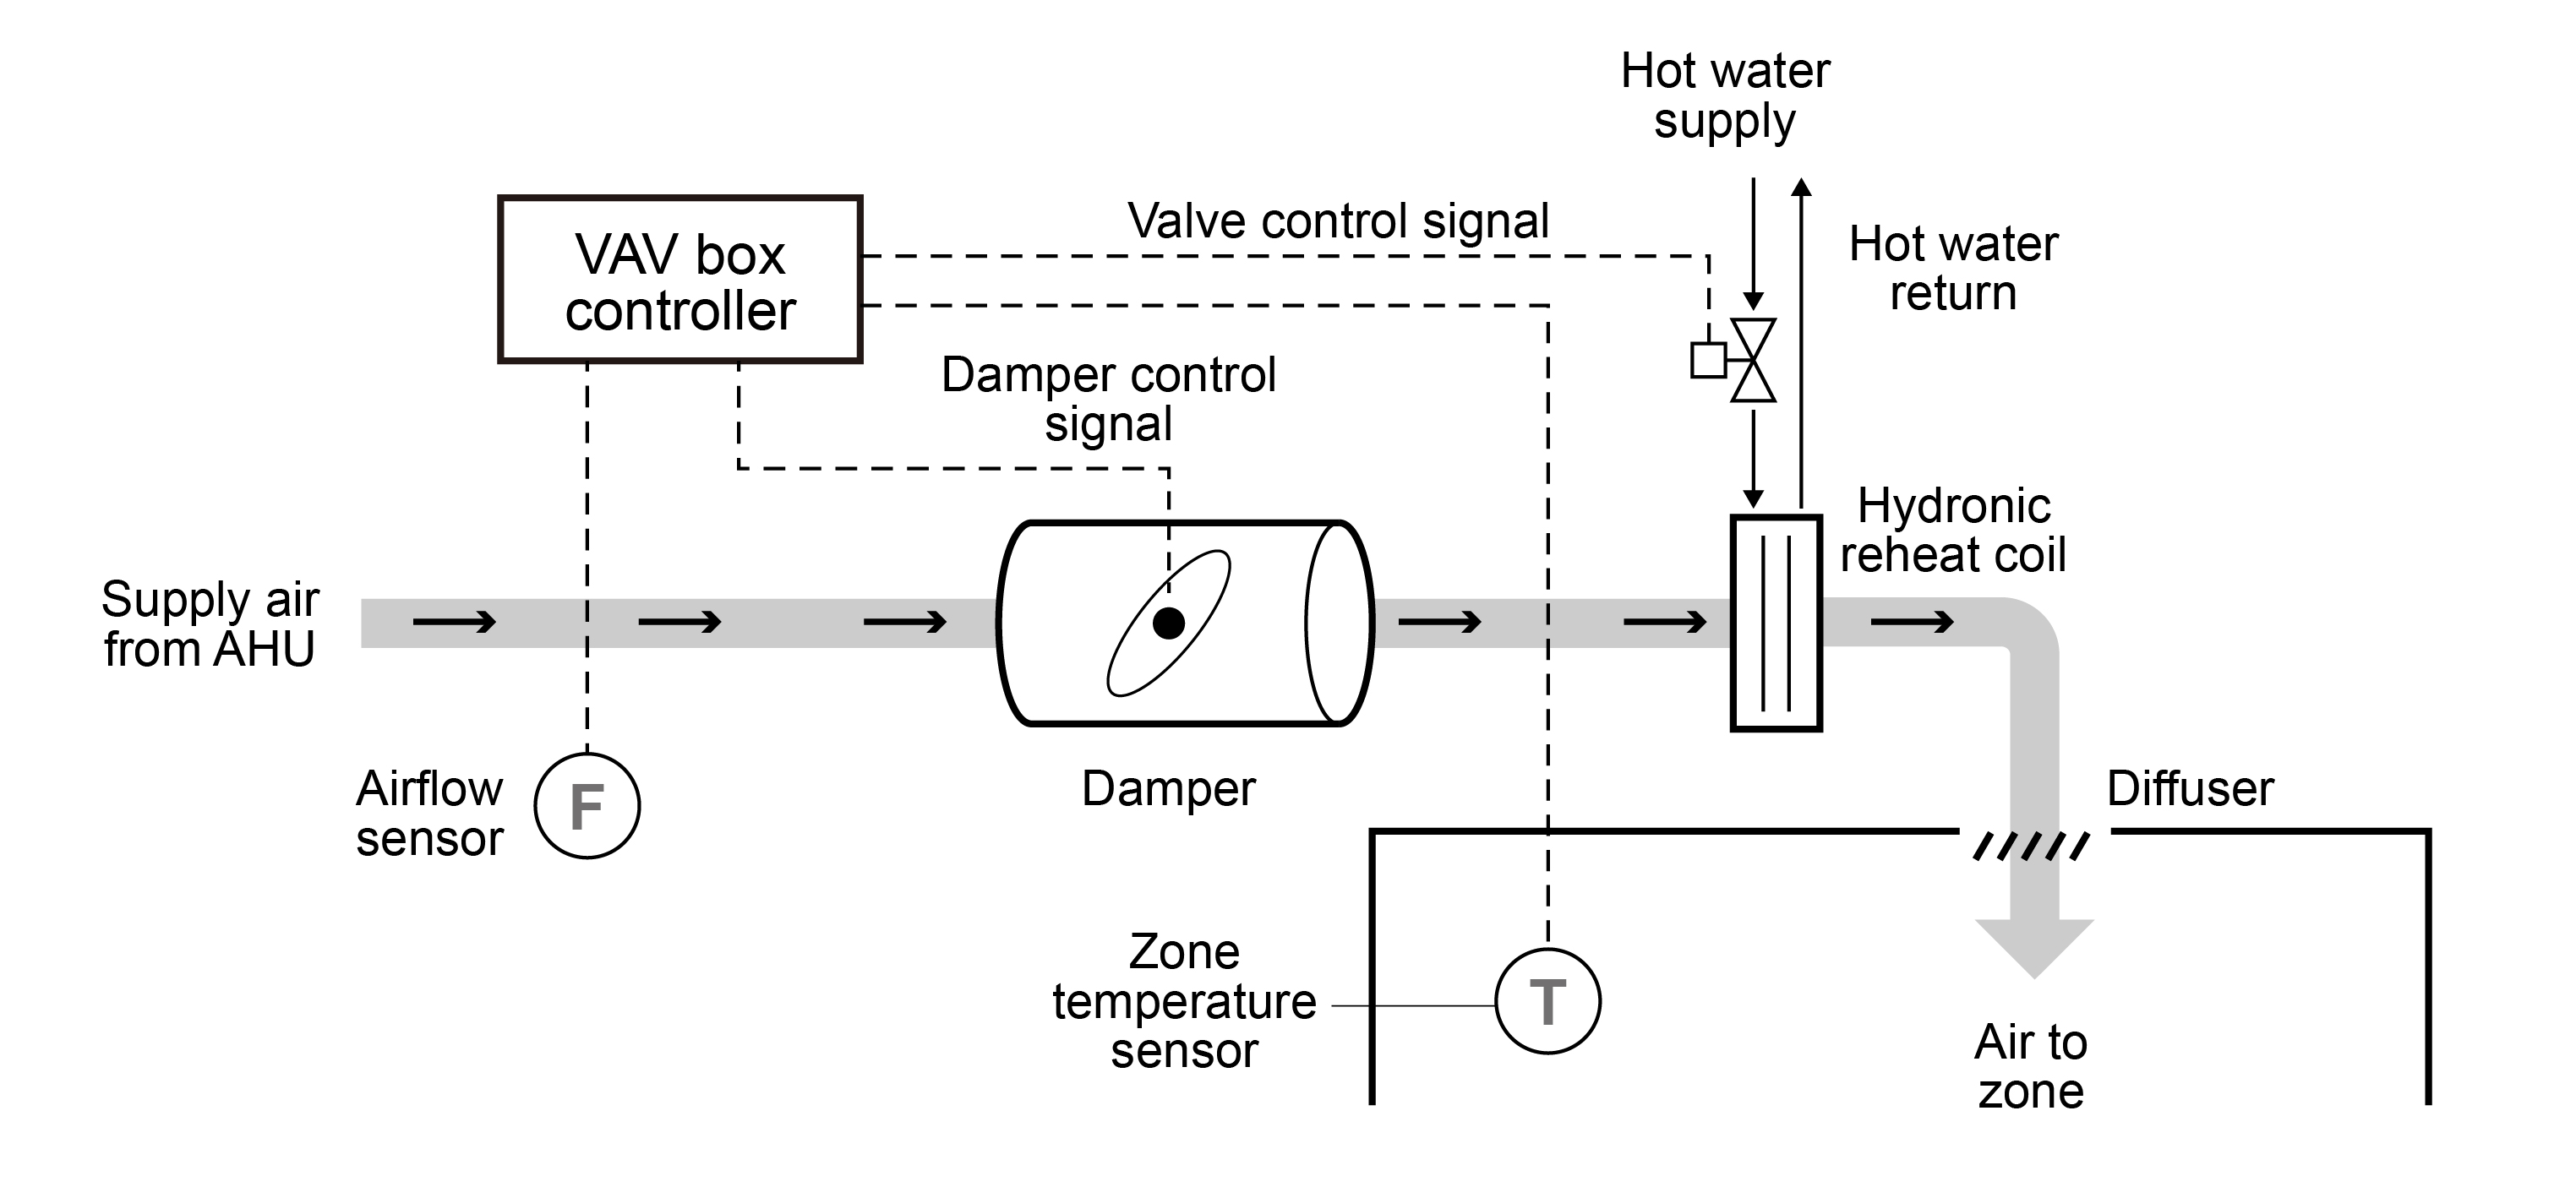
\includegraphics[width=0.5\textwidth]{Figures/VAV.jpeg}}
\caption{A detailed view of VAV reheat system.}
\label{fig2}
\end{figure}

Over the last few decades, the integration of building automation systems (BAS) has significantly lower the cost of data collection, storage, and commutation of building HVAC systems. It broadens the opportunities for the design and implementation of avant-garde control strategies. Although conventional controllers, such as on-off controls, model-free proportional-integral-derivative (PID) controls, and bang-bang controls are still widely used in small commercial buildings and residential buildings, researchers and engineers start to seek more sophisticated control strategies to handle the complexities, non-linearity, and disturbances in large-scale building HVAC systems. Particularly, model predictive control (MPC) has been extensively investigated given its ability to overcome the influence of time-varying disturbances, and its nature to work with slow motion dynamics by using optimization over a planning time window forward.

In some of the previous work trying to utilize MPC to optimize the energy usage as well as other related indices of HVAC, multiple objections are endeavored to minimize the tracking error and control effort. To summary, their objective functions are mostly one of or a combination of some of the following:
\begin{itemize}
\item Minimization of energy consumption and cost \cite{huang2015new,garnier2015predictive,kim2016simulation,lee2015optimal}.
\item Minimization of thermal discomfort hours\cite{asadi2014multi}.
\item Maintaining thermal comfort within range\cite{garnier2015predictive,kim2016simulation,ferreira2012neural}.
\item Maintaining Indoor Air Quality\cite{kusiak2011multi}.
\end{itemize}
If only one of the previous mentioned objective is included, the problem is known as a single objective optimization. On the other hand, if multiple objectives are used, the problem further changed to a multi-objective optimization.

Among different MPC implementation, one branch utilize the ability of Artificial Neural Network, which has been developed for different types of structures, mostly for the purposes of research, is called ANN-MPC. The structure includes, but not limited to, commercial university buildings \cite{he2014performance}, airport buildings \cite{huang2015new}, office buildings \cite{garnier2015predictive,kim2016simulation}. Conventional ANN models are normally to be used to predict certain parameters/output within the HVAC system. These metrics include, but not limited to, outside weather parameters (air temperature, air humidity \cite{ferreira2012neural,ruano2016imbpc}) , indoor air temperature \cite{ferreira2012neural,ruano2016imbpc}, energy consumption of different components (by VAV box \cite{kusiak2010modeling}, by HVAC system as a whole \cite{kusiak2014minimization}).The most normal type of ANN used is Multi-layer Perceptron (MLP). Due to the limited space, a more detailed introduction on MLP can be find in \cite{afram2017artificial}.

In recent years, researchers have started to explore other optimal control options, such as iterative learning control (ILC). ILC is traditionally used for improving transient responses and tracking performance for systems that executes identical or similar tasks multiple times \cite{bristow2006survey,ahn2x007iterative}. Differs from adaptive control and repetitive control, ILC modifies the reference control signal instead of the controller itself. More importantly, ILC takes advantage of information in each iteration of the repetitive task. The signals and systems are described as a lifted form by stacking all the states and controls over the finite time horizon of one iteration. These characteristics of ILC make it a suitable for building HVAC systems for several reasons. First, even though building HVAC systems exhibit time-varying uncertainties and are difficult to build precise mathematical models, the dynamics behind the systems are not changing rapidly, and controlling temperatures and mass flow rates to match their set-points are similar as tracking reference trajectories. Secondly, building HVAC systems are running in different modes on daily and seasonable basis. Within each mode, the set-points remain relatively constant. The switch between different modes. introduces transient responses. Additionally, the disturbances to building HVAC systems such as weather change and occupancy behaviors are fairly periodic and repetitive. 

Early implementations of ILC methods for building HVAC systems include reduction of tracking errors during the transient portion of static pressure tracking of water pumps and supply fans \cite{yan2010iterative}. Minakais, Mishra, and Wen apply ILC strategy to building temperature regulation in a simulation environment \cite{minakais2014groundhog} and find that the energy consumption of the building HVAC system increased as the temperature set-points are more tightly followed. A series of work \cite{peng2016iterative,peng2016optimization,peng2017constrained,peng2017distributed,peng2018concurrent,peng2019optimization}, by Peng and members in Mechanical Systems Control Lab in University of California, Berkeley, proposes a cooperative and distributed ILC design for a four-zone AHU-VAV reheat system considered control input constraints and global energy consumption optimization. Lu, Ai, and Li propose an active disturbance rejection based ILC strategy for a VAV sysetm built in a building energy simulation platform \cite{lu2018active}. However, most of the current research on ILC application on building HVAC systems are conducted in either simulation or test-beds. Real-world and larger-scale implementations are rarely found. In this work, we implement the proposed ILC design on models built by real-world data and conduct the numerical simulation on a large-scale thrity-two-zone AHU-VAV reheat system.

In this work, we propose a bi-level control strategy for building HVAC systems: at the top level, the control optimization of AHU is done by a ANN-MPC algorithm that uses an Artificial Neural Network to train on MPC-Simulated Control data. The final network/controller is able to directly interact with the system and imitate the performance of conventional MPC in some extent. At the bottom level, the temperature control of VAV boxes is achieved by an ILC controller design to ensure a tight room air temperature regulation to its set-point without significant increase of the energy consumption.


\section{ANN-MPC Problem Formulation}
\subsection{Approach of combining ANN and MPC}
Normally for a HVAC system optimal control problem, ANN (MLP) is embedded into MPC controller in one of the following ways:
\begin{itemize}
\item Use ANN to predict the dynamics of the HVAC system (more specifically, under context, AHU unit). Due to the introduction of non-linearity from activation function, this can be a highly efficient approach if the system is non-linear or disturbances-include. Under such circumstance, the controller used is not limited to MPC since ANN could potentially be viewed as a 'integrator' in linear dynamics case.
\item Use ANN to predict the control that the MPC controller would generate given the state(s) and disturbance(s). With this approach, MPC would mostly be used under the purpose of generating data used as training and testing set for ANN controller. After tuning hyper-parameters, the ANN controller could directly interact with the system. Although the training phase is done offline with simulated data, the implementation can be achieved online.
\item By combining the previous two approaches, two ANN would be connected in a cascade manner where the first ANN is used as a controller that serves the exact purpose as the second way. Another ANN, at the same time, serves as an 'integrator' to simulate the non-linear dynamics (most likely with disturbances).
\end{itemize}

The approach is adapted from the second approach, which uses MPC to generate data as the input (training and testing data) for ANN to further produce a ANN controller capable of substituting the MPC controller and directly interact with the system.

Due to the scale of this problem, a simple feed-forward Multi-layer Perceptron is used which takes the state of the first $N$ (horizon) states and random disturbances (Gaussian Distribution) as inputs and outputs the optimal control.

To be more specific, the whole procedure can be divided into three different phases:
\begin{itemize}
\item Data Generation: Simulate the MPC with different allowed combinations of the initial state (two variables) and store those data as the input towards the MLP structure.
\item ANN Training and Evaluation: Divide the previous data into 80/20 division and use the prior set of data to train the MLP. Different network structures and hyper-parameters are tuned for best performance. With respect to structures, a network structure of asymptotically decrease hidden layer size is finally chose ($100\Longrightarrow80\Longrightarrow60\Longrightarrow40$).\\
\item System Simulation: Simulate the ANN controller by connect the simulated system with ANN controller: Current state and future $N$ (horizon) disturbances are sent into the trained MLP as input and the network would output the optimal control.
\end{itemize}

\subsection{Data Generation with MPC}
To generate data, a formulation of AHU control problem is presented:
\begin{align}\label{annMpcJ}
\min_{x,u} \quad & \sum_{j=0}^{N}[\frac{1}{2} Q_{1j}(T_{RA,\text{ref}}-T_{RA})^{2} \\ \nonumber 
&+\frac{1}{2} Q_{2j}(\dot{m}_{RA,\text{ref}}-\dot{m}_{RA})^{2}] \\ \nonumber 
&+\sum_{j=0}^{N-1}[\frac{1}{2} R_{1j}(\Delta\beta)^{2} +\frac{1}{2} R_{1j}(\Delta T_{SA})^{2} \\ \nonumber 
&+ \frac{1}{2} R_{1j}(\Delta\dot{m}_{OA})^{2}] \\ \nonumber 
\end{align}
\begin{subequations}
\begin{align}\label{annHardBound1}
\textrm{s.t.} \quad & X_{lb} \leqslant X_{j} \leqslant X_{ub} \\ \label{annHardBound2}
& U_{lb} \leqslant U_{j} \leqslant U_{ub} \\  \label{annDyn}
& X(j+1) = \mathbf{A}X(j) + \mathbf{B}U(j) + \mathbf{C}W(j)
\end{align}
\end{subequations}
$T_{RA}$ - Temperature of return air (1st element in state) \\
$\dot{m_{RA}}$ - Flow rate of return air (2nd element in state) \\
$\beta$ - The mixing ratio of mixing air (1st element in control)\\
$T_{SA}$ - Temperature of supply air (2nd element in control)\\
$\dot{m}_{OA}$ - Flow rate of outside air (3rd element in control)\\

In the objective function (\ref{annMpcJ}), the aim is to minimize the energy consumption as well as optimize thermal comfort. (\ref{annHardBound1})(\ref{annHardBound2}) are two of the constraints on state and control variables while equation (\ref{annDyn}) states system's dynamics constraint. Note that the coefficient matrices are retrieved from \cite{liang2014modeling}.

\begin{figure}[htbp]
\centering
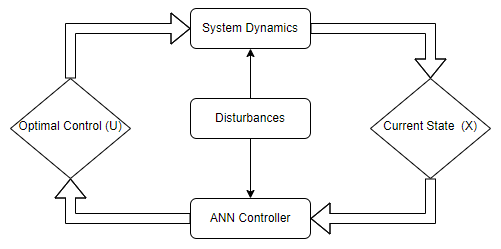
\includegraphics[width=0.5\textwidth]{Figures/ANN_Scheme.png}
\caption{ANN Simulation Scheme}
\label{fig:ANNmethod}
\end{figure}

\section{Dynamic modeling of VAV System} \label{thermalModeling}
In this section, we consider a well-known resistance-capacitance network \cite{gouda2000low}\cite{bueno2012resistance} for the room air temperature model. It assumes well-mixed room air in each thermal zone and a constant heat exchange rate between different thermal zones. If we have a building contains $n$ thermal zones, the thermal dynamics of zone $i$ can be expressed as
\begin{equation}
c_{i}\frac{dT_{i}}{dt}=\sum_{j=1}^{n}\frac{1}{R_{ji}}(T_{j}-T_{i})+u_{i}+w_{i}, \label{physics}
\end{equation}
where $c_{i}$ is the thermal capacitance of zone $i$, and $R_{ji}$ represents the thermal resistance of the heat exchange from zone $j$ to zone $i$. $T_{i}$ is the room air temperature of zone $i$, $u_{i}$ is the HVAC input, i.e. the discharge airflow from the VAV box, and $w_{i}$ is the thermal disturbances, such as outdoor weather and internal thermal load from occupants.

The control signal in (\ref{physics}) can be represented as
\begin{equation}
u_{i}=\dot{m_{da,i}}c_{p}(T_{da,i}-T_{i}), \label{control}
\end{equation}
where $\dot{m_{da,i}}$ and $T_{da,i}$ are the mass flow rate and temperature of the discharge air from the VAV box, respectively. The subscript $da$ represents the discharge air and $c_{p}$ is the specific heat capacity of air, which is assumed as constant ($1.012 J/(gK)$) for room temperature conditions.

If we discretize (\ref{physics}) at a sample time $t_{s}$ using forward difference:
\begin{align}
\nonumber 
T_{i}(k+1) &= T_{i}(k) + t_{s}(\sum_{j=1}^{n}\frac{1}{R_{ji}c_{i}}(T_{j}(k)-T_{i}(k))\\ \nonumber 
&+\frac{t_{s}}{c_{i}}u_{i}(k)+\frac{t_{s}}{c_{i}}w_{i}(k)\\ \nonumber
&= (1-\sum_{j=1}^{n}\frac{t_{s}}{R_{ji}c_{i}})T_{i}(k)+
\sum_{j=1}^{n}\frac{t_{s}}{R_{ji}c_{i}}T_{j}(k)\\ \label{digital}
&+\frac{t_{s}}{c_{i}}u_{i}(k)+\frac{t_{s}}{c_{i}}w_{i}(k)
\end{align}

Define the room temperature of $n$ thermal zones as the state vector:
\begin{equation}\label{t_vector}
    \mathbf{T}(k) = \begin{bmatrix}
        T_{1}(k) & T_{2}(k) & \cdots & T_{n}(k)  
    \end{bmatrix}^\top
\end{equation}
with a dimension of $n \times 1$. Since the HVAC input is designated for each zone, the control vector has the identical dimension of $n \times 1$:
\begin{equation}\label{u_vector}
    \mathbf{u}(k) = \begin{bmatrix}
        u_{1}(k) & u_{2}(k) & \cdots & u_{n}(k)  
    \end{bmatrix}^\top
\end{equation}
Similarly, we can have the disturbance vector as:
\begin{equation}\label{w_vector}
    \mathbf{w}(k) = \begin{bmatrix}
        w_{1}(k) & w_{2}(k) & \cdots & w_{n}(k)  
    \end{bmatrix}^\top
\end{equation}
If we re-write (\ref{digital}) in state space for $n$ thermal zones using (\ref{t_vector}), (\ref{u_vector}), and (\ref{w_vector}):
\begin{equation}\label{dyn_model}
    \mathbf{T}(k+1) = \mathbf{A}_{\textrm{v}}\mathbf{T}(k) + \mathbf{B}_{\textrm{v}}\mathbf{u}(k) + \mathbf{C}_{\textrm{v}}\mathbf{w}(k),
\end{equation}
where $\mathbf{A}_{\textrm{v}} = \mathbf{I_{n\times n}} - t_s (\mathbf{A_{1}} - \mathbf{A_{2}})$, and 
\begin{equation*}
\mathbf{A_{1}} = \left(\begin{IEEEeqnarraybox*}[][c]{,c/c/c,}
 a_{12}+\cdots+a_{1n} &  & \mathbf{0}\\
& \ddots &\\
\mathbf{0}&&a_{n1}+\cdots+a_{nn-1}%
\end{IEEEeqnarraybox*}\right),
\end{equation*}
\begin{equation*}
\mathbf{A_{2}} = \left(\begin{IEEEeqnarraybox*}[][c]{,c/c/c/c,}
0 & a_{12} & \cdots & a_{1n}\\
a_{21} & 0 & \cdots & a_{2n}\\
\vdots & \vdots & \ddots & \vdots\\
a_{n1} & a_{n2} & \cdots & 0%
\end{IEEEeqnarraybox*}\right).
\end{equation*}
The coefficient matrix $\mathbf{A}_{\textrm{v}}$ represents both the previous state and the heat transfer between different zones. For brevity, we use $a_{ji} = \frac{1}{R_{ji}c_{i}}$.

Also, for the coefficient matrix $\mathbf{B}_{\textrm{v}}$ for control is a diagonal matrix as the control input for each zone only applies to the zone itself:
\begin{equation*}
\mathbf{B}_{\textrm{v}} = \left(\begin{IEEEeqnarraybox*}[][c]{,c/c/c,}
\frac{1}{c_{1}} &  & \mathbf{0}\\
& \ddots &\\
\mathbf{0}&&\frac{1}{c_{n}}%
\end{IEEEeqnarraybox*}\right).
\end{equation*}
For the disturbance term, in this work, we are only using outsider air temperature as the thermal disturbance. The influence of occupancy behaviors will be investigated in future studies. Therefore, $w(k)$ is a time-varying scalar coefficient, $T_{oa}(k)$, where the subscript $oa$ represents outside air.
As a result, the coefficient matrix $\mathbf{C}_{\textrm{v}}$ can be written as:
\begin{equation*}
    \mathbf{C}_{\textrm{v}} = \begin{bmatrix}
         & \frac{1}{R_{oa,1}c_{1}} & \cdots & \frac{1}{R_{oa,i}c_{i}} & \cdots & \frac{1}{R_{oa,n}c_{n}}
    \end{bmatrix}^\top,
\end{equation*}
where $R_{oa,i}$ represents the heat exchange between zone $i$ and outdoor weather. Note that all the thermal zones in this work are exterior zones, which means they have at least one section of the perimeter that is adjacent to the outdoor.

We use real-world data for model identification. The model discrepancies by using forecast weather data as opposite using real-time outside air data will be discussed in Section \ref{discrepancy}.

To summarize this section, (\ref{dyn_model}) serves as the dynamic model used for ILC implementation in the next section.

\section{ILC Problem Formulation}
In this section, we present an ILC strategy for VAV-level temperature regulation. A room temperature set-point schedule $\mathbf{T}_{\textsuperscript{sp}}$ is retrieved from the real building HVAC system to serve as the reference state trajectory. The initial guess for the HVAC control input reference $\mathbf{u}_{\textsuperscript{ref}}$ is set as zero, since the it also represents the energy cost. In each roll-out, a QP-based MPC controller is used for objectives to follow the room temperature set-point reference trajectory and minimize the energy consumption. After each iteration, the reference trajectories of temperature and control input is updated based on an optimization-based ILC strategy.
\subsection{Baseline MPC Formulation}
In this section, we present a baseline QP-based MPC approach to solve the room temperature regulation problem in each roll-out. We have already developed the mathematical model for the room air temperature in Section \ref{thermalModeling}. It serves as the dynamic constraints in this MPC formulation.

For a prediction horizon $N$, we have the objective function:

\begin{align}
\nonumber
\min\limits_{\mathbf{u}}\frac{1}{2}\sum_{k=0}^{N}&(\mathbf{T}(k)-\mathbf{T}_{\text{sp}}(k))^\top\mathbf{Q}(\mathbf{T}(k)-\mathbf{T}_{\text{sp}}(k))\\
+ & (\mathbf{u}(k)-\mathbf{u}_{\textsuperscript{ref}}(k))^\top\mathbf{R}(\mathbf{u}(k)-\mathbf{u}_{\textsuperscript{ref}}(k)), \label{MinJ}%
\end{align}
\begin{subequations}
\begin{align}
\textrm{s.t.} \quad & \mathbf{u}_{\min}  \leq\mathbf{u}(k)\leq\mathbf{u}_{\max},\label{HardBounds}\\
&\mathbf{T}(k+1) = \mathbf{A}_{\textrm{v}}\mathbf{T}(k) + \mathbf{B}_{\textrm{v}}\mathbf{u}(k) + \mathbf{C}_{\textrm{v}}\mathbf{w}(k),\label{EqnofDynamicalConstraints}
\end{align}
\end{subequations}
where $\mathbf{T}_{\textsuperscript{sp}}(k)$ represents the set-point of room air temperature of each zone, and $\mathbf{Q}$ and $\mathbf{R}$ are the weighting coefficient matrices for the states and controls, respectively. (\ref{HardBounds}) represents the control limits of the VAV box, namely the maximum and minimum airflow rates that can be modulated by the control damper and the upper and lower bounds of discharge air temperature. (\ref{EqnofDynamicalConstraints}) is the dynamic constraint.

Note that the first term in (\ref{MinJ}) is used for temperature regulation, and the second term, also known as the control penalty term, acts as an energy usage indicator in a quadratic format. If we look at the physical meaning of the control input in (\ref{control}), it is the enthalpy change of the zone introduced by the HVAC system.

\subsection{ILC Iteration}
Given nominal trajectories $\mathbf{T}_{\textsuperscript{sp}}$ and $\mathbf{u}_{\textsuperscript{ref}}$ with a dynamic model formulated in Section \ref{thermalModeling} using forecast weather data $\mathbf{w}_\textsuperscript{fc}$, we use roll-outs on the real-time weather data $\mathbf{w}$ to find a $\Delta\mathbf{u}$ correction to $\mathbf{u}_{\textsuperscript{ref}}$ so that the actual system with real-time outdoor air temperature data $\mathbf{w}$ tracks the room temperature set-point $\mathbf{T}_{\textsuperscript{sp}}$ as closely as possible.

The objective function for the ILC formulation is:
\begin{align}
\nonumber
\min\limits_{\Delta\mathbf{u}}\frac{1}{2}\sum_{k=0}^{N}&(\Delta\mathbf{T}(k)-\Delta\tilde{\mathbf{T}}(k))^\top\mathbf{Q}_{\textsuperscript{ilc}}(\Delta\mathbf{T}(k)-\Delta\tilde{\mathbf{T}}(k))\\
+ & (\Delta\mathbf{u}(k)-\Delta\tilde{\mathbf{u}}(k))^\top\mathbf{R}_{\textsuperscript{ilc}}(\Delta\mathbf{u}(k)-\Delta\tilde{\mathbf{u}}(k)), \label{DeltaJ}%
\end{align}
\begin{subequations}
\begin{align}
\textrm{s.t.} \quad & \Delta\mathbf{u}_{\min}\leq\Delta\mathbf{u}(k)\leq\Delta\mathbf{u}_{\max},\label{DeltaBounds}\\
&\Delta\mathbf{T}(k+1) = \mathbf{A}_{\textrm{v}}\Delta\mathbf{T}(k) + \mathbf{B}_{\textrm{v}}\Delta\mathbf{u}(k) + \mathbf{C}_{\textrm{v}}\Delta\mathbf{w}(k),\label{DeltaEqnofDynamicalConstraints}
\end{align}
\end{subequations}
where $\Delta\mathbf{T} = \mathbf{T} - \mathbf{T}_{\textsuperscript{sp}}$, $\tilde{\mathbf{T}}$ is the temperature trajectory from the model running on real-world outdoor air temperature data. After every iteration, the reference controls $\mathbf{u}_{\textsuperscript{ref}}$ are updated using $\Delta\mathbf{u}$. $\mathbf{Q}_{\textsuperscript{ilc}}$ and $\mathbf{R}_{\textsuperscript{ilc}}$ are the weighting coefficient matrices for the states and controls in the ILC formulation, respectively.

Note that we also compute $\Delta\mathbf{w} = \mathbf{w}_\textsuperscript{fc} - \mathbf{w}$, which is the difference between the forecast temperature data and the real-time outside air data.

\section{Numerical Results}
In this section, we demonstrate the model identification and control simulation with extensive measurements from an office building on the campus of the University of California, Merced (UC Merced). Historical data between May 1st to May 31st, 2014 were collected, cleansed, and pre-processed by one of the author's previous thesis work \cite{liang2014modeling}. The HVAC control system in the building obeys the communication protocol for building automation and control networks (BACnet) by ASHRAE, ANSI and ISO standard \cite{bushby1997bacnettm}. The online data storage and direct digital control (DDC) are accessible by a BAS interface, WebCTRL$\textsuperscript{\textregistered}$ \cite{webctrl2022alc}.

To validate the models in this work, we first select a series of metrics for evaluating the accuracy of validation. In literature regarding data analysis of time series in building science and technology area \cite{FraustoPietersDeltour03,Anderson94,Brillinger01,NorgaardRavnPoulsenHansen00,Norlen90}, it is common to use $\mathrm{MAE}$, $\mathrm{MSE}$, $\mathrm{RMSE}$, coefficient of determination ($r^{2}$) and maximum absolute error ($\mathrm{MaxAE}$). 
These are defined as
\begin{align}
&\mathrm{MAE}=\frac{1}{m}\underset{i=1}{\overset{m}{\sum}}\left\vert X_{i}%
-X_{i}^{\ast}\right\vert ,\\
&\mathrm{MSE}=\frac{1}{m}\underset{i=1}{\overset{m}{\sum}}(X_{i}-X_{i}^{\ast}%
)^{2},\\
&\mathrm{RMSE}=[\frac{1}{m}\underset{i=1}{\overset{m}{\sum}}(X_{i}-X_{i}^{\ast
})^{2}]^{1/2},\\
&r^{2}=\frac{(m\sum X_{i}X_{i}^{\ast}-(\sum X_{i})(\sum X_{i}^{\ast}%
))^{2}}{(m(\sum X_{i}^{2})-(\sum X_{i})^{2})(m(\sum X_{i}^{\ast2})-(\sum
X_{i}^{\ast})^{2})},\\
&\mathrm{MaxAE}=\underset{i}{\max}\left\vert X_{i}-X_{i}^{\ast}\right\vert ,
\end{align}
where $X_{i}$, and $X_{i}^{\ast}$ are the estimated values and measurements of
a particular attribute in the time domain, respectively, and $m$ is the total
number of measurements.

\subsection{ANN-MPC Results}
\subsubsection{Evaluation on test dataset}
The first set of metrics used to evaluate the performance of ANN-MPC is done on the $20\%$ of data used as testing dataset (MAE and MSE are calculated on the control output from the ANN-MPC controller and the conventional MPC controller, batch-wise):
\begin{itemize}
\item Accuracy: $99.13\%$ 
\item MAE: 7.89
\item MSE: 321.34
\end{itemize}

The training phase of the controller is stopped at an MAE of 7.

\subsubsection{Evaluation through simulation}
Although the final accuracy on testing dataset is acceptable to some extent, the ultimate purpose of this controller is to directly interact with the system and perform online optimal control. So the next test we perform is to initiate a simulation with disturbances with the same level of magnitude as those training dataset (Fig. \ref{fig_RA_ANN}, Fig. \ref{fig_SA_ANN}).

\begin{figure}[htbp]
\centerline{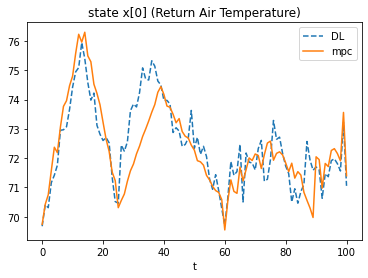
\includegraphics[width=0.5\textwidth]{Figures/Return_Air_Temperature.png}}
\caption{The simulated return air temperature (which is the first scalar within the size two state vector) with MPC controller and ANN-MPC controller with a random initial state at a disturbance magnitude of 5}
\label{fig_RA_ANN}
\end{figure}

\begin{figure}[htbp]
\centerline{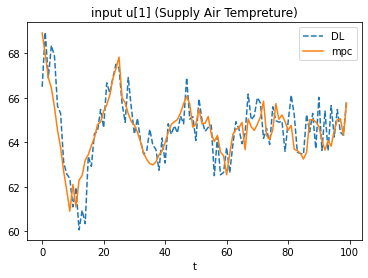
\includegraphics[width=0.5\textwidth]{Figures/Supply_Air_Temperature.png}}
\caption{The simulated supply air temperature (which is the second scalar within the size three control vector) with MPC controller and ANN-MPC controller with a random initial state at a disturbance magnitude of 5}
\label{fig_SA_ANN}
\end{figure}


\begin{table}[htbp]
\caption{The metrics of return air temperature between ANN-MPC and conventional MPC over 50 simulations at a disturbance level of 2, 5 and 10, instance-wise.}
\begin{center}
\begin{tabular}{|c|c|c|c|}
\hline
\textbf{Disturbance} &\multicolumn{3}{|c|}{\textbf{Metrics}} \\
\cline{2-4} 
\textbf{Level}&\textbf{MAE} & \textbf{MSE} & \textbf{RMSE}  \\
\hline
disturbance 2 & 0.7209 & 0.8491 & 0.7360
\\
disturbance 5 & 0.7330 & 0.8561 & 0.7385
\\
disturbance 10 & 0.7595 & 0.8715 & 0.7749\\
\hline
\end{tabular}
\label{tab_ANN_Dis}
\end{center}
\end{table}

The results clearly show that the action taken by the ANN-MPC controller is less optimal through simulation since bound conditions are often violated for different important parameters: the return air temperature, for example, goes below the lower bound. Another fact to notice is that, when the disturbance level is further increased to $10$ or decrease to $2$, the previously mentioned behavior (higher tracking error as the system evolves) remains (Table \ref{tab_ANN_Dis}).

\subsection{ILC Results}
\subsubsection{Dynamic Model Identification}
Measurements from thirty-two VAVs under one AHU are available for the development of the RC model of room air temperature during May 2014. For zone $i$ at time step $k$, the measurements include room air temperature $T_{i}(k)$, the set-point of the room air temperature $T_{\text{sp},i}(k)$, the discharge mass airflow rate $\dot{m}_{da,i}$, the discharge air temperature $T_{da,i}$. Additionally, the real-time outside air temperature data $T_{oa}(k)$ was measured by the weather station near the outside air inlet of the AHU. All the aforementioned measurements have been collected over 26 days with a sampling interval of 15 minutes. Note that the operation differences between occupied hours (6am-0am on weekdays) and occupied hours (weekends, holidays, and other hours) of the building HVAC system is significant. Besides, temperature regulation should be more strictly enforced during the occupied hours as it matters the thermal comfort of the occupants. In this work, we partition the measurements by occupied and unoccupied hours and only use the data that fall in the occupied mode for modeling and control.

The coefficient matrices $\mathbf{A}_{\textrm{v}}$, $\mathbf{B}_{\textrm{v}}$, and $\mathbf{C}_{\textrm{v}}$ in (\ref{dyn_model}) are identified with the method of least square \cite{WuSun12}. In this section, two models are developed using the identical model structure:
\begin{itemize}
\item \textbf{\textit{Forecast Model}}: This model is trained using the building HVAC data and forecast outside air temperature data. The historical forecast outside air data of the weather station located closest to UC Merced campus is retrieved from World Weather Online $\textsuperscript{\textregistered}$ \cite{wwo2022api} website using their Python-based API. For the model validation, the real-time data takes the place of the forecast data for outside air temperature. The remaining data items remain unchanged.
\item \textbf{\textit{Real-time Model}}: This model is both trained and validated using the building HVAC data and real-time outside air temperature data.
\end{itemize}

Table \ref{tabModel} presents the validation errors of several rooms using the real-time model. Due to the format limitation, we only show the results four rooms for best and worst validation results. It can be seen that the tracking error is small and consistent among all the zones except Room 16. In fact, Room 16 is an outlier given its raw data quality. The data imputation performed in \cite{liang2014modeling} may not be able to capture the actual dynamics of the VAV box serving that zone.

\begin{table}[htbp]
\caption{The errors of selected room temperature models.}
\begin{center}
\begin{tabular}{|c|c|c|c|c|c|}
\hline
\textbf{Room} &\multicolumn{5}{|c|}{\textbf{Metrics}} \\
\cline{2-6} 
\textbf{Number}&\textbf{MAE} & \textbf{MSE} & \textbf{RMSE} & $r^2$ & \textbf{MaxAE} \\
\hline
Room 2$^{\mathrm{a}}$ &  0.0419  &  0.0044  &  0.0666 &  0.9949  &  1.1215\\
Room 32$^{\mathrm{a}}$ & 0.0329  &  0.0030  &  0.0545  &  0.9942 &   1.3426\\
Room 9$^{\mathrm{b}}$ & 0.0339  & 0.0027  & 0.0518 &  0.9440  & 0.5340\\
Room 16$^{\mathrm{b}}$ & 0.0865 &  0.0194  & 0.1393  & 0.8124 & 0.9292 \\
\hline
\multicolumn{4}{l}{$^{\mathrm{a}}$The models with most accuracy.}\\
\multicolumn{4}{l}{$^{\mathrm{a}}$The models with least accuracy..}
\end{tabular}
\label{tabModel}
\end{center}
\end{table}

\subsubsection{Model Discrepancies} \label{discrepancy}

Fig. \ref{figModel} presents a one-day room air temperature validation of the forecast model and real-time model of Room 29. It is observed that the validation of the real-time model, shown in magenta solid line, matches well with the measured room air temperature. In the other hand, the forecast model that is validated with real-time outside air data, shown in red dot line, displays an obvious offset to the ground truth value.

\begin{figure}[htbp]
\centerline{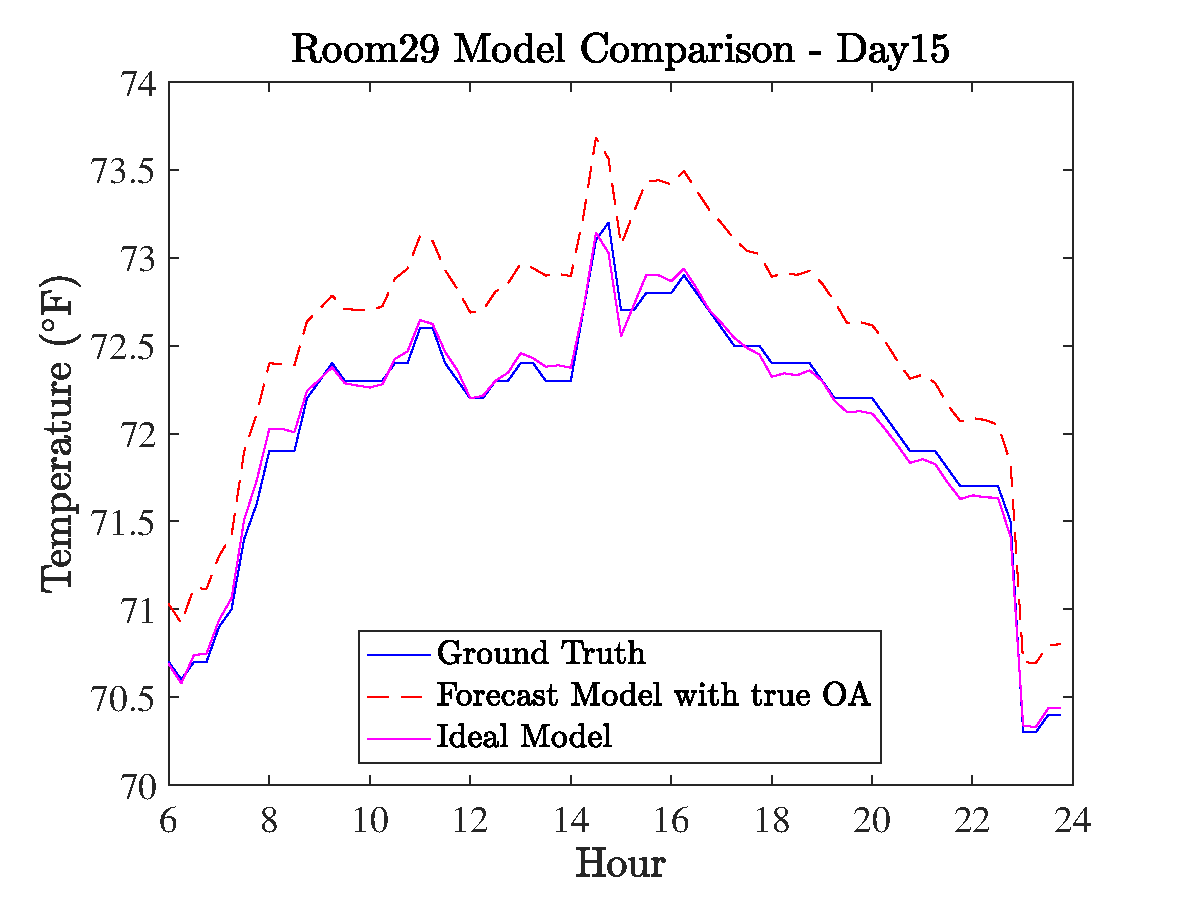
\includegraphics[width=0.5\textwidth]{Figures/three_models.eps}}
\caption{A one-day (Day 15) comparison between test results of the ground truth of room air temperature, the model trained with forecast data but tested with real-time data, and the model trained and tested with real-time data of Room 29.}
\label{figModel}
\end{figure}

Table \ref{tabModelDis} shows the comparison of the average validation errors between the forecast model and real-time model of the thirty-two zones. It is expected that the coefficient of determination $r^2$ does not vary substantially because even though the forecast outside air data are not accurate, it still exhibits a similar pattern to the real-time outside air data that indicates a strong correlation to the room air temperature data. However, it can be seen that the $\mathrm{MAE}$ and $\mathrm{MSE}$ are significantly increased from the real-time model to the forecast model. It implies that the tracking error of the forecast model is remarkably larger than that of the real-time model.

\begin{table}[htbp]
\caption{The metrics of room temperature model validation between forecast model and real-time model.}
\begin{center}
\begin{tabular}{|c|c|c|c|c|c|}
\hline
\textbf{Model} &\multicolumn{5}{|c|}{\textbf{Metrics}} \\
\cline{2-6} 
\textbf{Trained with}&\textbf{MAE} & \textbf{MSE} & \textbf{RMSE} & $r^2$ & \textbf{MaxAE} \\
\hline
Forecast Data & 0.1227  &  0.0253  &  0.1380 &   0.9726  &  0.8877
\\
Real-time Data & 0.0455  &  0.0057 &  0.0698 &  0.9732 &  0.8637 \\
\hline
\end{tabular}
\label{tabModelDis}
\end{center}
\end{table}

With regard to the differences of the disturbances, the weather forecast data and real-time outside air data are shown in Fig. \ref{figOA}. It is observed that the disturbances are non-repetitive and there are uncertainties in the differences.

\begin{figure}[htbp]
\centerline{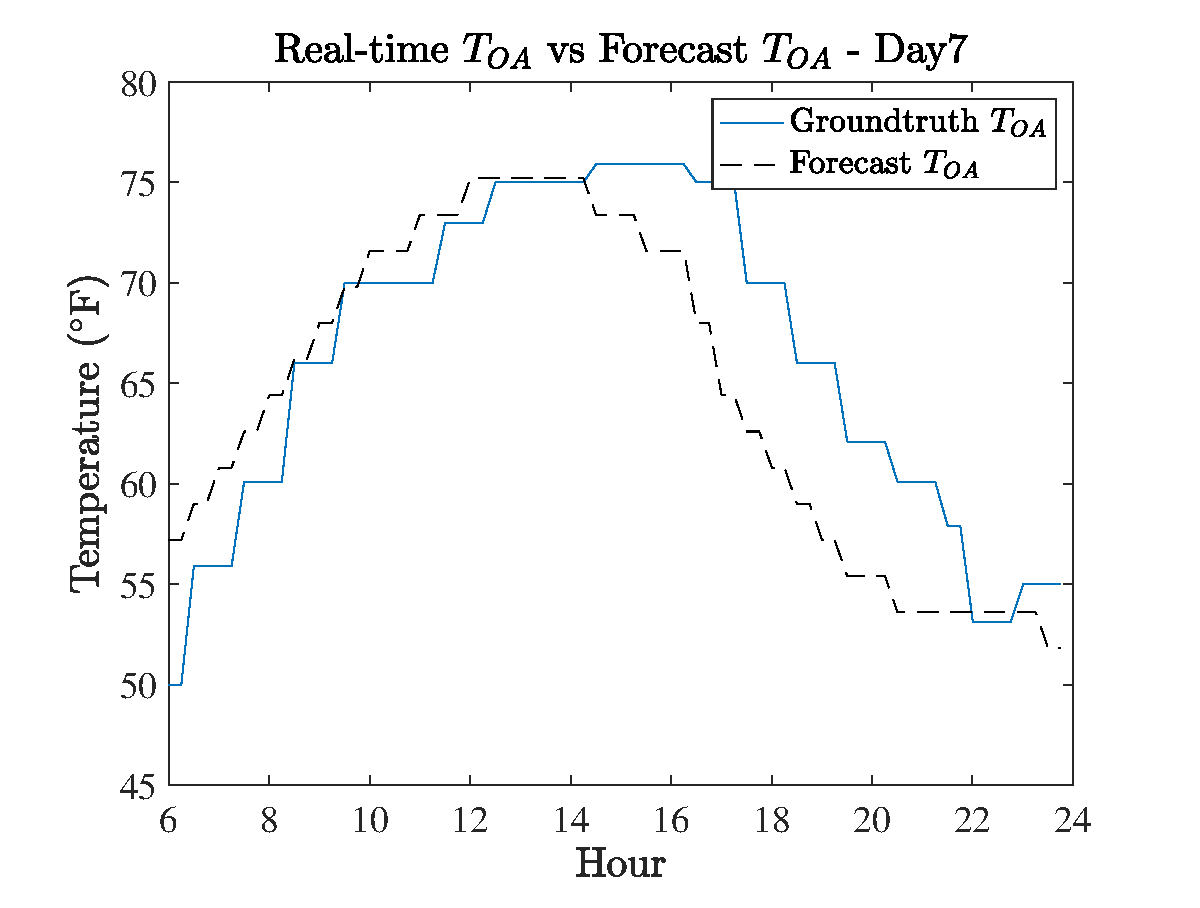
\includegraphics[width=0.5\textwidth]{Figures/oa_comp.eps}}
\caption{Differences between forecast and measured outside air temperature data.}
\label{figOA}
\end{figure}

In the following control simulation, the forecast model will be used as the inexact model for the ILC formulation. Using weather forecast data is a highly plausible scenario for real-world deployment of this control framework since it is impossible to retrieve future "real-time" weather data.

\subsubsection{Control Simulation Results}
In this section, numerical simulation results are displayed to demonstrate the effectiveness of the ILC control strategy. The identical data used in the model identification are also used for control simulation. 

The set-points data and control limits are collected from the BAS database and/or construction documents of the building. The ILC controller is computed after a one-day roll-out, meaning thatg one iteration is one-day length, eighteen hours with 72 data points. The MPC controller within each roll-out is computed based on an one hour, namely 4 data points.

Fig. \ref{figILC1} shows the room air temperature trajectories of Room 1 from Day 1 to Day 8. It is observed that the temperature dynamics converge to the set-point trajectory in 2 to 3 iterations. It should be noted that for Room 1, from Day 7 there is an abrupt change of the room air temperature set-point from 72.5$^\circ$F to 74$^\circ$F. The ILC controller is capable to capture this alteration and responses quickly. The system trajectory re-converge to the new set-point in 2 iterations. The temperature profiles reveal that the system performance has been notably improved with the non-receptive outside air temperature data uncertainty. 

\begin{figure}[htbp]
\centerline{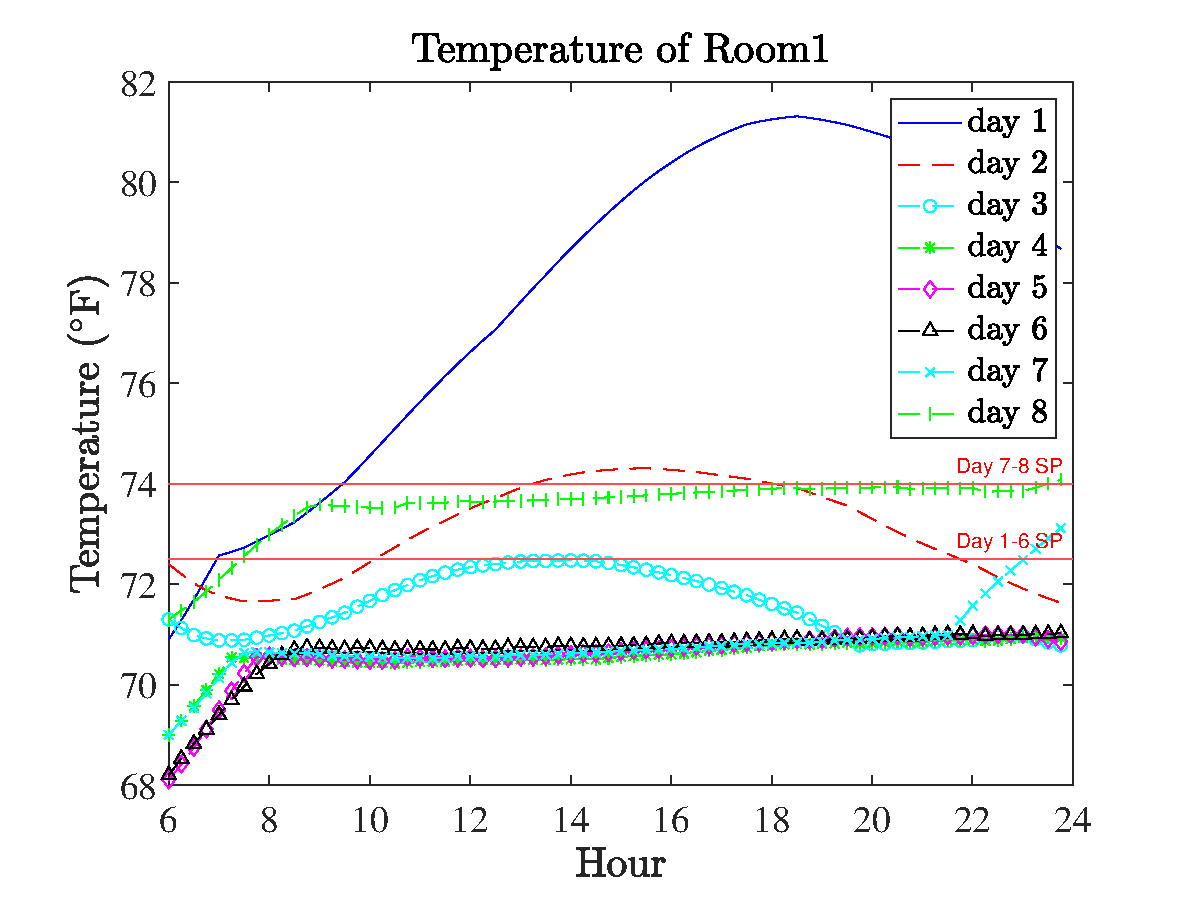
\includegraphics[width=0.5\textwidth]{Figures/ilc_results.eps}}
\caption{Temperature profiles of Room 1 in 8 Days.}
\label{figILC1}
\end{figure}

Fig. \ref{figILC1C} shows the control signals of Room 1 from Day 1 to Day 8. It can be seen that the control lower and upper bound are strictly enforced. Compared to the first iteration, the later iterations modified the control signals in warm-up hours of the occupied mode. It indicates that the system needs to put more control effort in early hours of the daytime to ensure that the room air temperature follows the set-point. It implies a slight increase of energy consumption, but it is the trade-off for a more tight temperature regulation.

\begin{figure}[htbp]
\centerline{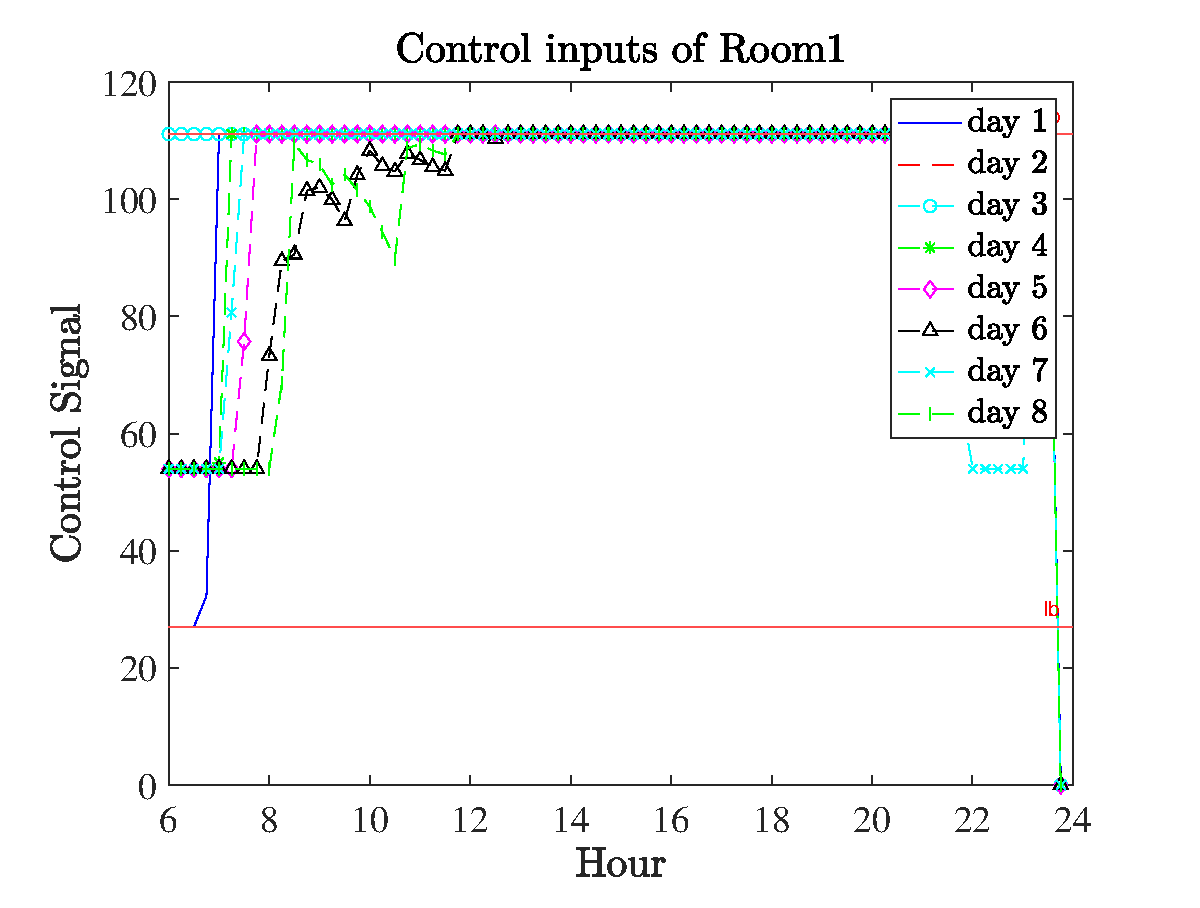
\includegraphics[width=0.5\textwidth]{Figures/ilc_control.eps}}
\caption{Control signals of Room 1 in 8 Days.}
\label{figILC1C}
\end{figure}

\section{Conclusions}
We proposed a deep learning based MPC controller to produce optimal control for AHU that utilize the outputs from conventional MPC controller within system simulation with disturbances. The result indicates that the deep learning based controller is able to show an acceptable tracking performance in limited simulations.

We also propose a QP-based ILC controller with room air temperature set-points reference, and HVAC control saturation constraints. A thirty-two-zone VAV system achieves tight tracking performance to its set-points without a significant increase of the energy consumption. 

For future work, we would like to develop a top-down hierarchical controller by linking the bi-level control design together. Additionally, more disturbances to building HVAC systems, such as occupancy behaviors and partial failure of the systems will be studied to establish the effectiveness of the proposed ILC design. With respect to the ANN-MPC, future endeavors could be done on either training the dataset to a lower metric or on a different architecture (e.g. Long short-term memory, LSTM). However, if other architectures are implemented, it is essential to consider the possibility and performance of its online control.
\section*{Acknowledgment}

We would like to thank Dr. Zachary Manchester and all the teaching staff of 16745 course for all the patience and help throughout this semester. We also want to thank Yiting Zhang from School of Architecture for drawing HVAC system diagrams for this work.

% \begin{thebibliography}{00}
% \bibitem{b1} G. Eason, B. Noble, and I. N. Sneddon, ``On certain integrals of Lipschitz-Hankel type involving products of Bessel functions,'' Phil. Trans. Roy. Soc. London, vol. A247, pp. 529--551, April 1955.
% \bibitem{b2} J. Clerk Maxwell, A Treatise on Electricity and Magnetism, 3rd ed., vol. 2. Oxford: Clarendon, 1892, pp.68--73.
% \bibitem{b3} I. S. Jacobs and C. P. Bean, ``Fine particles, thin films and exchange anisotropy,'' in Magnetism, vol. III, G. T. Rado and H. Suhl, Eds. New York: Academic, 1963, pp. 271--350.
% \bibitem{b4} K. Elissa, ``Title of paper if known,'' unpublished.
% \bibitem{b5} R. Nicole, ``Title of paper with only first word capitalized,'' J. Name Stand. Abbrev., in press.
% \bibitem{b6} Y. Yorozu, M. Hirano, K. Oka, and Y. Tagawa, ``Electron spectroscopy studies on magneto-optical media and plastic substrate interface,'' IEEE Transl. J. Magn. Japan, vol. 2, pp. 740--741, August 1987 [Digests 9th Annual Conf. Magnetics Japan, p. 301, 1982].
% \bibitem{b7} M. Young, The Technical Writer's Handbook. Mill Valley, CA: University Science, 1989.
% \end{thebibliography}

\bibliographystyle{IEEEtran}
\bibliography{IEEEabrv,ref16745}

\end{document}
